% !TEX encoding = UTF-8 Unicode

\documentclass[a4paper]{article}

\usepackage{color}
\usepackage{xcolor}
\usepackage{url}
\usepackage[T2A]{fontenc} % enable Cyrillic fonts
\usepackage[utf8]{inputenc} % make weird characters work
\usepackage{graphicx}
\usepackage{amsthm}
\usepackage{amsmath}
\usepackage{amsfonts}
\usepackage{booktabs,hhline}
\usepackage{caption}
\usepackage{subcaption}

\usepackage{multirow}       % used for making multirow tables (Nemanja)

%\usepackage[english,serbian]{babel}
\usepackage[english,serbianc]{babel} %ukljuciti babel sa ovim opcijama, umesto gornjim, ukoliko se koristi cirilica

\usepackage[unicode]{hyperref}
\hypersetup{colorlinks,citecolor=green,filecolor=green,linkcolor=blue,urlcolor=blue}

\newtheorem{primer}{Пример}[section] %ćirilični primer
%\newtheorem{primer}{Primer}[section]

\newtheorem{definic}{Дефиниција}
\newcommand{\norm}[1]{\left\lVert#1\right\rVert}

\begin{document}

\title{Решавање неких логичких игара користећи \textsc{smt} решаваче\\ \small{Семинарски рад у оквиру курса\\Аутоматско резоновање\\ Математички факултет}}

\author{Немања Мићовић, Лазар Ранковић\\nmicovic@outlook.com, lazar.rankovic@outlook.com}
\date{}
\maketitle

\abstract{
    Логичке игре дуги низ година поседују велику дозу занимљивости и представљају чест хоби.
    Како комплексност логичких игара може бити висока, јавља се проблем прављења логичких игара и генерисање
    њиховог почетног стања за које
    смо сигурни да постоји решење и да је јединствено.
    Рад разматра примену \textsc{smt} решавача за верификацију решења логичких игара и доказивање јединствености решења.
    Показује се да су се \textsc{smt} решавачи показали као одличан алат за решавање поменутих проблема јер природно описују
    ограничења која постоје у логичким играма.
}

\tableofcontents

\newpage
% ---------------------------------------------------------------------------------------------------------------------
\section{Увод}
\label{sec:intro}
% ---------------------------------------------------------------------------------------------------------------------
Deo \ref{sec:logicGames} говори o логичким играма и илуструје неке од популарнијих.

У делу \ref{sec:smtSolver} даје се кратак историјски преглед релевантних историјских догађа,
уводи се концепт \textsc{sat} и \textsc{smt} решавача.
Део \ref{sec:logicSmt} приказује пример решавања једне од познатих логичких игара користећи \textsc{smt} решавач.

% ---------------------------------------------------------------------------------------------------------------------
\section{Логичке игре}
\label{sec:logicGames}
% ---------------------------------------------------------------------------------------------------------------------
Логичке игре за собом имају дубоку традицију и историју, а упркос страховито брзом развоју технологије у последњих
неколико година, и даље поседују велику популарност. Разлог за њихову популарност јесте често једноставност правила,
вежбање људског ума и неочекивана комплекност решавања која уме да заинтригира људе.
У многим часописима се редовно штампају игре као што је судоку (приказан на слици \ref{fig:sudoku}). 

Пре неколико година појавила се игра 2048 (слика \ref{fig:2048} у којој корисник може да помера поља хоризонтално или вертикално.
При померању, сва поља се померају и транслирају се док не ударе у зид или друго поље. Када се поља са истим бројевима
сударе, они постају једно поље које представља њихов збир. Играч је победио када
у игри успе да конструише поље чија је вредност 2048. Игра је преузета преко 20 милиона пута са \emph{Google Play} и \emph{iTunes}
продавница за мобилне уређаје.

Логичке игре односно загонетке су погодне за математички опис користећи логику и представљају чест пример примене
\textsc{sat} и \textsc{smt} решавача за генерисање инстанци проблема, решавање и валидацију да ли је решење јединствено.

\begin{figure}
\centering
\begin{minipage}{.5\textwidth}
    \centering
    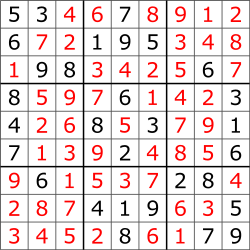
\includegraphics[width=.4\linewidth]{./slike/sudoku.png}
    \captionof{figure}{Игра Судоку}
    \label{fig:sudoku}
\end{minipage}%
\begin{minipage}{.5\textwidth}
  \centering
  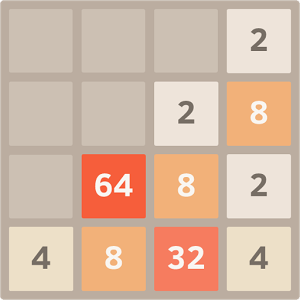
\includegraphics[width=.4\linewidth]{./slike/2048.png}
  \captionof{figure}{Игра 2048}
  \label{fig:2048}
\end{minipage}
\end{figure}


% ---------------------------------------------------------------------------------------------------------------------
\section{\textsc{smt} решавачи}
\label{sec:smtSolver}
% ---------------------------------------------------------------------------------------------------------------------
\subsection{Кратак преглед релеватних историјских догађаја}
Готфрид Вилхелм Лајбниц\footnote{Gottfried Wilhelm Leibniz (1646-1716)} је међу првима изнео идеју
о механизацији процеса људског резоновања.

Године 1928. Давид Хилберт\footnote{David Hilbert (1862-1943)} је поставио проблем одлучивања - \emph{Entscheidungsproblem}.
Проблем тражи алгоритам који узима као улаз формулу логике првог реда и одговара ДА или НЕ да ли је формула универзално
тачна или не.

Алонзо Черч\footnote{Alonzo Church (1903-1995)} и Алан Тјуринг\footnote{Alan Turing (1912-1954)} у засебним радовима 1936. године показују да опште решење за Хилбертов проблем одлучивања
не постоји. Черч доказ изводи свођењем на ламбда рачун, а Алан Тјуринг редукцијом на халтинг проблем.

Но показује се да уколико се извши рестрикција на одређену теорију, ипак можемо добити многе одлучиве фрагменте теорије логике
првог реда и често је управо ту примена \textsc{smt} решавача.

Крајем 20. и почетком 21. века велика популарност проблема задовољивости исказних формула (проблем \textsc{sat}) доводи до развоја
ефикаснијих и драстично бржих алгоритама решавања \cite{satcdcl1, satcdcl2, satcdcl3}. Иако је проблем \textsc{np} комплетан,
\textsc{sat} решавачи могу решавати и формуле које имају чак и десетине хиљада променљивих. Наравно, постоје формуле које ће изазвати
експоненцијално понашање алгоритма који имплементира решавач.

Популарност проблема \textsc{sat} и постојање ефикасних алгоритама за његово решавање
природно води у идеју да се конструишу решавачи који ће бити у бити у стању да решавају
формуле логике првог реда. Како логика првог реда није одлучива поставља се питање да ли се може
редуковати скуп дозвољених симбола, ограничити домен тако да се добије одлучива теорија?
Показује се да је одговор да, део \ref{subsubsec:theories} илуструје неке од теорија.
Настаје нова врста решавача који се називају \textsc{smt} (eng. Satisfiability Modulo Theories) и нова област \textsc{smt}.

\subsection{\textsc{smt} решавач}
\textsc{smt} решавачи су засновани на \textsc{sat} решавачима и поседују виши степен апстракције чиме задржавају и семантику која се
налази у формули. То омогућава и примену специјализованих алгоритама који могу узети додатну семантику у обзир.

\textsc{smt} решавачи имају модуларну архитектуру (слика \ref{fig:smtarch}) која се најчешће састоји из два централна дела,
\textsc{cdcl} (eng. Conflict Driven Clause Learning) заснован \textsc{sat} решавач \cite{satcdcl1, satcdcl2, satcdcl3} и \textsc{smt} језгро
које имплементира неки од решавача за конкретну теорију (део \ref{subsubsec:theories}) који се најчешће назива \textsc{T} решавач.
При промени теорије над којом се резонује, модуларни приступ
омогућава да се задржи део система који се бави решавање проблема \textsc{sat}.

\begin{figure}
    \centering
    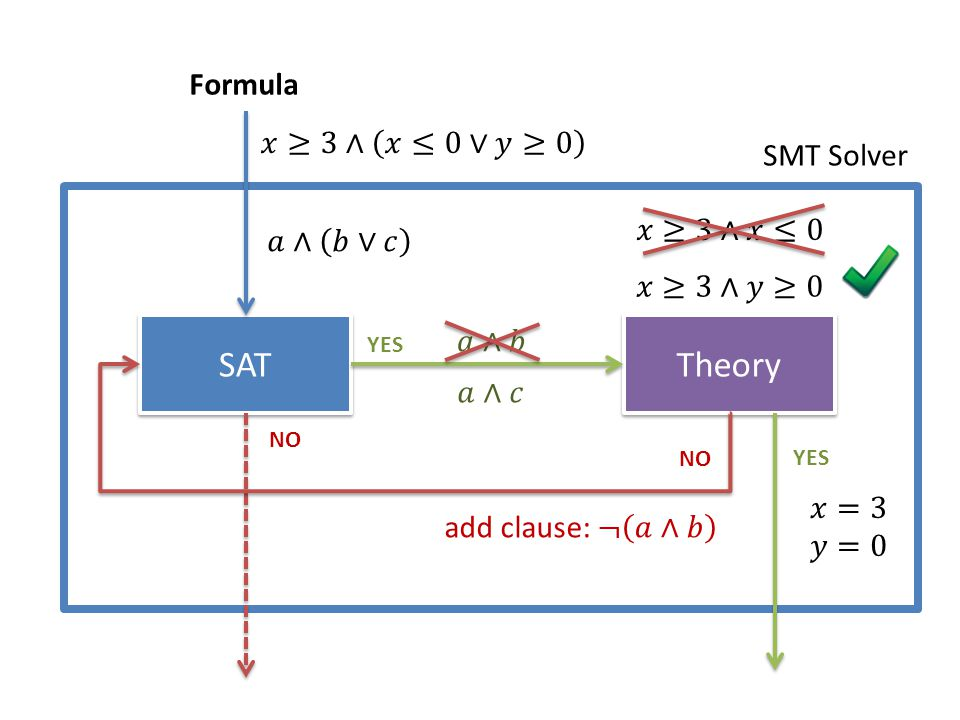
\includegraphics[width=.7\linewidth]{./slike/arch.jpg}
    \captionof{figure}{Архитектура \textsc{smt} решавача}
    \label{fig:smtarch}
\end{figure}

\subsection{Примене \textsc{smt} решавача}
\textsc{smt} решавачи имају широку примену у области верификације софтвера и хардвера \cite{smtexample1, smtexample2, smtexample3, smtexample4},
но корисни су и у другим ситуацијама у којима је формула логике првог реда редукована на неку теорију адекватна за опис проблема.


Једна од примена \textsc{smt} решавача јесу и логичке игре где се \textsc{smt} решавач може користити за генерисање инстанци игре,
генерисање решења игре, провере да ли је решење тачно као и доказ да је решење игре јединствено. У делу
\ref{sec:logicSmt} биће приказана примена \textsc{smt} решавача над једном логичком игром.


\subsubsection{Неке од коришћених теорија}
\label{subsubsec:theories}

Постоји више развијених теорија насталих за разне домене примена \textsc{smt} решавача.
Неке од њих су:
\begin{itemize}
    \item \textsc{euf} теорија
    \item реална аритметика
    \item целобројна аритметика
    \item теорија низова
    \item теорија битвектора
\end{itemize}

\paragraph{\textsc{euf} теорија} \textsc{euf} (eng. Equality with Uninterpreted Functions) теорија је теорија која садржи
један предикатски симбол, симбол једнакости = и произвољан број сорти
и функцијских симбола који се могу поптупно слободно интерпретирати.
\textsc{smt} проблем за ову теорију је неодличив, но базни фрагмент теорије је одлучив. Задовољивост коњункције базних литерала
је одлучив у полиномијалном времену користећи Нелсон-Open процедуру \cite{handbookar}.


\paragraph{Реална аритметика} Теорија која описује реалну аритметику поседује сорту \emph{Real} и симболе
0, 1, +, $\cdot$, -, /, $\leq$. Модел теорије је структура реалних бројева $\mathbb{R}$. Теорија је одлучива,
а проблем испитивања задовољивости коњункције линеарних базних литерала је одлучив у полиномијалном времену.
Користе се Фурије-Моцкинова процедура \cite{handbookar} и Симплекс процедура \cite{lp}.

\paragraph{Целобројна аритметика} Теорија описује целобројну аритметику, поседује сорту \emph{Int} и симболе
0, 1, +, $\cdot$, -, $\leq$. Модел теорије је структура целих бројева $\mathbb{Z}$. У општем случају теорија је
неодлучива, но њен линеарни фрагмент (Презбургерова аритметика \cite{handbookar}) је одлучив. Проблем испитивања
задовољивости коњункције линеарних базних литерала је одлучив и \textsc{np} комплетан.

\paragraph{Теорија низова} Теорија низова се користи за апстракцију концепта низа. Поседује сорте
\emph{Array}, \emph{Index} и \emph{Value} који представљају, редом, низ, индекс низа и вредност коју елементи
низа могу узимати. Симболи \emph{select} и \emph{store} апстрахују индексирање низа и додељивање вредности
елементу низа. Приметимо да се неће мењази вредности низа при операцији \emph{store} већ ће операција
враћати нови низ који настане када се у оригиналном низу промени вредност.
Теорија је неодлучива у општем случају, но базни фрагмент теорије је одлучив. Проблем испитивања
задовољивости коњункције базних литерала је \textsc{np} комплетан.

\paragraph{Теорија битвектора} Теорија битвектора се користи за опис бинарних бројева и има значајну примену
у области верификације хардвера. Теорија је одлучива, а проблем испитивања задовољивости коњункције базних
литерала је \textsc{np} комплетан.

% ---------------------------------------------------------------------------------------------------------------------
\section{Решавање логичких игара користећи \textsc{smt} решаваче}
\label{sec:logicSmt}
% ---------------------------------------------------------------------------------------------------------------------
У овом делу ће бити изложен пример решавања логичке игре коришћењем \textsc{Yices} \textsc{smt} решавача \cite{yices}.

% -------------------------------------------------------------------------------------------------
\subsection{Логичка игра Три суседне}
% -------------------------------------------------------------------------------------------------
Логичка игра \emph{Три судедне} се састоји из матрице поља димензије $n \times n$. На почетку игре,
поља су обојена у плаво, бело и сиво. Ово ћемо називати \emph{почетно стање игре}.
Поља која су обојена у сиво, играч може да промени у плава или бела произвољан број пута,
док оригинална плава и бела поља не може да мења. 
Циљ игре је да играч сва сива поља означи као плава или бела при чему морају да важе следећа ограничења:
\begin{itemize}
    \item Не постоје три суседна поља у истој врсти која су обојена истом бојом (услов 1)
    \item Не постоје три суседна поља у истој колони која су обојена истом бојом (услов 2)
    \item У свим врстама мора бити једнак број плавих и белих поља (услов 3)
    \item У свим колонама мора бити једнак број плавих и белих поља (услов 4)
\end{itemize}

Стање у којем се налази табла (матрица) игре када је игра решена називаћемо \emph{задовољено стање игре}.

На слици \ref{fig:threeway_original} је приказанo почетно стање игре, а на слици \ref{fig:threeway_solved} решена инстанца игре игрe \emph{Три суседне}.

\begin{figure}
\centering
\begin{minipage}{.5\textwidth}
    \centering
    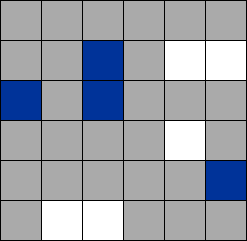
\includegraphics[width=.4\linewidth]{./slike/three_way_original.png}
    \captionof{figure}{Почетно стање игре}
    \label{fig:threeway_original}
\end{minipage}%
\begin{minipage}{.5\textwidth}
  \centering
  
\includegraphics[width=.4\linewidth]{./slike/three_way_solved.png}
  \captionof{figure}{Задовољено стање игре}
  \label{fig:threeway_solved}
\end{minipage}
\end{figure}

\subsubsection{Огранињења}
Како би \textsc{smt} решавачем генерисали решења биће нам потребно кодирање претходно наведених услова. Таблу игре
ћемо кодирати користећи $n \times n$ променљивих које ћемо означавати са $x_{i, j}$.

\[
    x_{i, j} = \left\{\begin{array}{lr}
        \, -1, & \text{за бела поља} \\
        \quad 0, & \text{за сива поља } \\
        \quad 1, & \text{за плава поља }
    \end{array}\right\}
\]

При чему важи:
$$ I = \{0, 1, ..., n-1\} $$
$$ J = \{0, 1, ..., n-1\} $$
$$ T = \{-2, -1, 0, 1, 2\} $$
$$ i \in I, j \in J $$

Са $i$ ћемо означавати индекс врсте, при чему $i= 0$ означава прву врсту, а $i = n-1$ означава последњу врсту. Аналогно за  $j$,
$ј = 0$ означава прву колону, а  $j = n-1$ последњу колону.


\paragraph{Услов 1}
Кодирање услова 1 изводимо захтевом да збир три суседна поља у врсти мора припадати скупу $T$. Како имамо $n$ врсти,
при чему по свакој врсти имамо $n-2$ ограничења, добијамо $n(n-2)$ ограничења.

$$ x_{i,j} + x_{i, j+1} + x_{i, j+2} \in T $$
$$ i \in \{0, 1, ..., n-1\} $$
$$ j \in \{0, 1, ..., n-3\} $$

\paragraph{Услов 2}
Услов 2 је симетричан услову 1 тако да се добија још $n(n-2)$ додатних ограничења облика:
$$ x_{i, j} + x_{i+1, j} + x_{i+2, j} \in T $$
$$ i \in \{0, 1, ..., n-3\} $$
$$ j \in \{0, 1, ..., n-1\} $$

\paragraph{Услов 3}
Намећемо ограничење да збир у свакој врсти мора бити 0. Како променљиве $x_{i, j}$ имају вредност 1 или -1, ограничење
имплицира једнак број плавих и белих поља у врсти. Ако је број врсти $n$ тиме добијамо још $n$ ограничења облика:
$$ x_{0, 0} + x_{0, 1} + ... + x_{0, n-1} = 0 $$
$$ x_{1, 0} + x_{1, 1} + ... + x_{1, n-1} = 0 $$
$$ ...  $$
$$ x_{n-1, 0} + x_{n-1, 1} + ... + x_{n-1, n-1} = 0 $$

\paragraph{Услов 4}
Услов 4 је симетричан услову 3 те добијамо додатних $n$ ограничења облика:
$$ x_{0, 0} + x_{0, 1} + ... + x_{0, n-1} = 0 $$
$$ x_{0, 1} + x_{1, 1} + ... + x_{n-1, 1} = 0 $$
$$ ...  $$
$$ x_{0, n-1} + x_{1, n-1} + ... + x_{n-1, n-1} = 0 $$

\paragraph{Услови домена}
Решавачу је потребно наметнути дозвољене вредности за сваку од променљивих. Како решавање логичке игре започињемо
од унапред задатог стања (нека поља су већ обојена и не могу се мењати), имамо две врсте ограничења.

Оригинално задата плава и бела поља, решавачу намећемо вредности променљивих 1 или -1. Ако је на пример
поље (0, 3) обојено у плаво, а поље (3, 2) у бело мора важити:
$$ x_{0, 3} = 1 $$
$$ x_{3, 2} = -1 $$

За свако сиво обојено поље $x_{i, j}$, намећемо ограничења да вредности могу бити или -1 или 1.
$$
    x_{i, j} \neq 0 \land -1 \geq x_{i, j} \leq 1
$$

Како имамо $n \times n$ променљивих, добијамо још $n \times n$ услова.

\paragraph{Сложеност проблема} За игру димензије $n$ из претходно изложеног добијамо укупно $3n^2 - 2n$ услова.
Дакле број услова квадратно зависи од димензије $n$ и асимптотски се понаша као $O(n^2)$.

\subsubsection{Питање јединствености решења}
Како би се показала и доказала јединственост решењa, може се користити решавач да се добију вредности променљивих, а да се након тога
додају ограничења да променљиве не могу узети вредности које представљају решења. Овде треба бити опрезан и приметити да само оригинална сива
поља треба ограничити, а плава и бела (из почетног стања игре) не.

\subsection{Yices program}
Написан је c++ програм који за дато почетно стање игре генерише претходно наведена ограничења у синтакси погодној за
yices \textsc{smt} решавач. Следи генерисани код за једну од инстанци игре.

\begin{verbatim}
(set-logic QF_LIA)
(declare-fun x0_0 () Int)
(declare-fun x0_1 () Int)
(declare-fun x0_2 () Int)
(declare-fun x0_3 () Int)
(declare-fun x0_4 () Int)
(declare-fun x0_5 () Int)
(declare-fun x1_0 () Int)
(declare-fun x1_1 () Int)
(declare-fun x1_2 () Int)
(declare-fun x1_3 () Int)
(declare-fun x1_4 () Int)
(declare-fun x1_5 () Int)
(declare-fun x2_0 () Int)
(declare-fun x2_1 () Int)
(declare-fun x2_2 () Int)
(declare-fun x2_3 () Int)
(declare-fun x2_4 () Int)
(declare-fun x2_5 () Int)
(declare-fun x3_0 () Int)
(declare-fun x3_1 () Int)
(declare-fun x3_2 () Int)
(declare-fun x3_3 () Int)
(declare-fun x3_4 () Int)
(declare-fun x3_5 () Int)
(declare-fun x4_0 () Int)
(declare-fun x4_1 () Int)
(declare-fun x4_2 () Int)
(declare-fun x4_3 () Int)
(declare-fun x4_4 () Int)
(declare-fun x4_5 () Int)
(declare-fun x5_0 () Int)
(declare-fun x5_1 () Int)
(declare-fun x5_2 () Int)
(declare-fun x5_3 () Int)
(declare-fun x5_4 () Int)
(declare-fun x5_5 () Int)
(assert
    (and
        ;; Ограничења домена
        (and (<= (- 1) x0_0)(>= 1 x0_0)(distinct 0 x0_0))
        (and (<= (- 1) x0_1)(>= 1 x0_1)(distinct 0 x0_1))
        (= x0_2 1)
        (and (<= (- 1) x0_3)(>= 1 x0_3)(distinct 0 x0_3))
        (and (<= (- 1) x0_4)(>= 1 x0_4)(distinct 0 x0_4))
        (and (<= (- 1) x0_5)(>= 1 x0_5)(distinct 0 x0_5))
        (and (<= (- 1) x1_0)(>= 1 x1_0)(distinct 0 x1_0))
        (= x1_1 1)
        (and (<= (- 1) x1_2)(>= 1 x1_2)(distinct 0 x1_2))
        (and (<= (- 1) x1_3)(>= 1 x1_3)(distinct 0 x1_3))
        (= x1_4 (- 1))
        (and (<= (- 1) x1_5)(>= 1 x1_5)(distinct 0 x1_5))
        (and (<= (- 1) x2_0)(>= 1 x2_0)(distinct 0 x2_0))
        (= x2_1 (- 1))
        (and (<= (- 1) x2_2)(>= 1 x2_2)(distinct 0 x2_2))
        (and (<= (- 1) x2_3)(>= 1 x2_3)(distinct 0 x2_3))
        (and (<= (- 1) x2_4)(>= 1 x2_4)(distinct 0 x2_4))
        (and (<= (- 1) x2_5)(>= 1 x2_5)(distinct 0 x2_5))
        (= x3_0 (- 1))
        (and (<= (- 1) x3_1)(>= 1 x3_1)(distinct 0 x3_1))
        (= x3_2 1)
        (and (<= (- 1) x3_3)(>= 1 x3_3)(distinct 0 x3_3))
        (= x3_4 (- 1))
        (and (<= (- 1) x3_5)(>= 1 x3_5)(distinct 0 x3_5))
        (and (<= (- 1) x4_0)(>= 1 x4_0)(distinct 0 x4_0))
        (and (<= (- 1) x4_1)(>= 1 x4_1)(distinct 0 x4_1))
        (and (<= (- 1) x4_2)(>= 1 x4_2)(distinct 0 x4_2))
        (and (<= (- 1) x4_3)(>= 1 x4_3)(distinct 0 x4_3))
        (and (<= (- 1) x4_4)(>= 1 x4_4)(distinct 0 x4_4))
        (= x4_5 (- 1))
        (and (<= (- 1) x5_0)(>= 1 x5_0)(distinct 0 x5_0))
        (= x5_1 1)
        (= x5_2 1)
        (and (<= (- 1) x5_3)(>= 1 x5_3)(distinct 0 x5_3))
        (= x5_4 1)
        (and (<= (- 1) x5_5)(>= 1 x5_5)(distinct 0 x5_5))

        ;; У истој врсти три суседна поља не смеју бити сте боје
        (and (> (+ x0_0 x0_1 x0_2) (- 3))(< (+ x0_0 x0_1 x0_2) 3))
        (and (> (+ x0_0 x0_1 x0_2) (- 3))(< (+ x0_0 x0_1 x0_2) 3))
        (and (> (+ x0_1 x0_2 x0_3) (- 3))(< (+ x0_1 x0_2 x0_3) 3))
        (and (> (+ x0_1 x0_2 x0_3) (- 3))(< (+ x0_1 x0_2 x0_3) 3))
        (and (> (+ x0_2 x0_3 x0_4) (- 3))(< (+ x0_2 x0_3 x0_4) 3))
        (and (> (+ x0_2 x0_3 x0_4) (- 3))(< (+ x0_2 x0_3 x0_4) 3))
        (and (> (+ x0_3 x0_4 x0_5) (- 3))(< (+ x0_3 x0_4 x0_5) 3))
        (and (> (+ x0_3 x0_4 x0_5) (- 3))(< (+ x0_3 x0_4 x0_5) 3))
        (and (> (+ x1_0 x1_1 x1_2) (- 3))(< (+ x1_0 x1_1 x1_2) 3))
        (and (> (+ x1_0 x1_1 x1_2) (- 3))(< (+ x1_0 x1_1 x1_2) 3))
        (and (> (+ x1_1 x1_2 x1_3) (- 3))(< (+ x1_1 x1_2 x1_3) 3))
        (and (> (+ x1_1 x1_2 x1_3) (- 3))(< (+ x1_1 x1_2 x1_3) 3))
        (and (> (+ x1_2 x1_3 x1_4) (- 3))(< (+ x1_2 x1_3 x1_4) 3))
        (and (> (+ x1_2 x1_3 x1_4) (- 3))(< (+ x1_2 x1_3 x1_4) 3))
        (and (> (+ x1_3 x1_4 x1_5) (- 3))(< (+ x1_3 x1_4 x1_5) 3))
        (and (> (+ x1_3 x1_4 x1_5) (- 3))(< (+ x1_3 x1_4 x1_5) 3))
        (and (> (+ x2_0 x2_1 x2_2) (- 3))(< (+ x2_0 x2_1 x2_2) 3))
        (and (> (+ x2_0 x2_1 x2_2) (- 3))(< (+ x2_0 x2_1 x2_2) 3))
        (and (> (+ x2_1 x2_2 x2_3) (- 3))(< (+ x2_1 x2_2 x2_3) 3))
        (and (> (+ x2_1 x2_2 x2_3) (- 3))(< (+ x2_1 x2_2 x2_3) 3))
        (and (> (+ x2_2 x2_3 x2_4) (- 3))(< (+ x2_2 x2_3 x2_4) 3))
        (and (> (+ x2_2 x2_3 x2_4) (- 3))(< (+ x2_2 x2_3 x2_4) 3))
        (and (> (+ x2_3 x2_4 x2_5) (- 3))(< (+ x2_3 x2_4 x2_5) 3))
        (and (> (+ x2_3 x2_4 x2_5) (- 3))(< (+ x2_3 x2_4 x2_5) 3))
        (and (> (+ x3_0 x3_1 x3_2) (- 3))(< (+ x3_0 x3_1 x3_2) 3))
        (and (> (+ x3_0 x3_1 x3_2) (- 3))(< (+ x3_0 x3_1 x3_2) 3))
        (and (> (+ x3_1 x3_2 x3_3) (- 3))(< (+ x3_1 x3_2 x3_3) 3))
        (and (> (+ x3_1 x3_2 x3_3) (- 3))(< (+ x3_1 x3_2 x3_3) 3))
        (and (> (+ x3_2 x3_3 x3_4) (- 3))(< (+ x3_2 x3_3 x3_4) 3))
        (and (> (+ x3_2 x3_3 x3_4) (- 3))(< (+ x3_2 x3_3 x3_4) 3))
        (and (> (+ x3_3 x3_4 x3_5) (- 3))(< (+ x3_3 x3_4 x3_5) 3))
        (and (> (+ x3_3 x3_4 x3_5) (- 3))(< (+ x3_3 x3_4 x3_5) 3))
        (and (> (+ x4_0 x4_1 x4_2) (- 3))(< (+ x4_0 x4_1 x4_2) 3))
        (and (> (+ x4_0 x4_1 x4_2) (- 3))(< (+ x4_0 x4_1 x4_2) 3))
        (and (> (+ x4_1 x4_2 x4_3) (- 3))(< (+ x4_1 x4_2 x4_3) 3))
        (and (> (+ x4_1 x4_2 x4_3) (- 3))(< (+ x4_1 x4_2 x4_3) 3))
        (and (> (+ x4_2 x4_3 x4_4) (- 3))(< (+ x4_2 x4_3 x4_4) 3))
        (and (> (+ x4_2 x4_3 x4_4) (- 3))(< (+ x4_2 x4_3 x4_4) 3))
        (and (> (+ x4_3 x4_4 x4_5) (- 3))(< (+ x4_3 x4_4 x4_5) 3))
        (and (> (+ x4_3 x4_4 x4_5) (- 3))(< (+ x4_3 x4_4 x4_5) 3))
        (and (> (+ x5_0 x5_1 x5_2) (- 3))(< (+ x5_0 x5_1 x5_2) 3))
        (and (> (+ x5_0 x5_1 x5_2) (- 3))(< (+ x5_0 x5_1 x5_2) 3))
        (and (> (+ x5_1 x5_2 x5_3) (- 3))(< (+ x5_1 x5_2 x5_3) 3))
        (and (> (+ x5_1 x5_2 x5_3) (- 3))(< (+ x5_1 x5_2 x5_3) 3))
        (and (> (+ x5_2 x5_3 x5_4) (- 3))(< (+ x5_2 x5_3 x5_4) 3))
        (and (> (+ x5_2 x5_3 x5_4) (- 3))(< (+ x5_2 x5_3 x5_4) 3))
        (and (> (+ x5_3 x5_4 x5_5) (- 3))(< (+ x5_3 x5_4 x5_5) 3))
        (and (> (+ x5_3 x5_4 x5_5) (- 3))(< (+ x5_3 x5_4 x5_5) 3))

        ;; У истој колони три суседна поља не смеју бити сте боје
        (and (> (+ x0_0 x1_0 x2_0) (- 3))(< (+ x0_0 x1_0 x2_0) 3))
        (and (> (+ x1_0 x2_0 x3_0) (- 3))(< (+ x1_0 x2_0 x3_0) 3))
        (and (> (+ x2_0 x3_0 x4_0) (- 3))(< (+ x2_0 x3_0 x4_0) 3))
        (and (> (+ x3_0 x4_0 x5_0) (- 3))(< (+ x3_0 x4_0 x5_0) 3))
        (and (> (+ x0_1 x1_1 x2_1) (- 3))(< (+ x0_1 x1_1 x2_1) 3))
        (and (> (+ x1_1 x2_1 x3_1) (- 3))(< (+ x1_1 x2_1 x3_1) 3))
        (and (> (+ x2_1 x3_1 x4_1) (- 3))(< (+ x2_1 x3_1 x4_1) 3))
        (and (> (+ x3_1 x4_1 x5_1) (- 3))(< (+ x3_1 x4_1 x5_1) 3))
        (and (> (+ x0_2 x1_2 x2_2) (- 3))(< (+ x0_2 x1_2 x2_2) 3))
        (and (> (+ x1_2 x2_2 x3_2) (- 3))(< (+ x1_2 x2_2 x3_2) 3))
        (and (> (+ x2_2 x3_2 x4_2) (- 3))(< (+ x2_2 x3_2 x4_2) 3))
        (and (> (+ x3_2 x4_2 x5_2) (- 3))(< (+ x3_2 x4_2 x5_2) 3))
        (and (> (+ x0_3 x1_3 x2_3) (- 3))(< (+ x0_3 x1_3 x2_3) 3))
        (and (> (+ x1_3 x2_3 x3_3) (- 3))(< (+ x1_3 x2_3 x3_3) 3))
        (and (> (+ x2_3 x3_3 x4_3) (- 3))(< (+ x2_3 x3_3 x4_3) 3))
        (and (> (+ x3_3 x4_3 x5_3) (- 3))(< (+ x3_3 x4_3 x5_3) 3))
        (and (> (+ x0_4 x1_4 x2_4) (- 3))(< (+ x0_4 x1_4 x2_4) 3))
        (and (> (+ x1_4 x2_4 x3_4) (- 3))(< (+ x1_4 x2_4 x3_4) 3))
        (and (> (+ x2_4 x3_4 x4_4) (- 3))(< (+ x2_4 x3_4 x4_4) 3))
        (and (> (+ x3_4 x4_4 x5_4) (- 3))(< (+ x3_4 x4_4 x5_4) 3))
        (and (> (+ x0_5 x1_5 x2_5) (- 3))(< (+ x0_5 x1_5 x2_5) 3))
        (and (> (+ x1_5 x2_5 x3_5) (- 3))(< (+ x1_5 x2_5 x3_5) 3))
        (and (> (+ x2_5 x3_5 x4_5) (- 3))(< (+ x2_5 x3_5 x4_5) 3))
        (and (> (+ x3_5 x4_5 x5_5) (- 3))(< (+ x3_5 x4_5 x5_5) 3))

        ;; За сваку врсту мора постојати једнак број плавих и белих поља.
        (= 0 (+ x0_0 x0_1 x0_2 x0_3 x0_4 x0_5))
        (= 0 (+ x1_0 x1_1 x1_2 x1_3 x1_4 x1_5))
        (= 0 (+ x2_0 x2_1 x2_2 x2_3 x2_4 x2_5))
        (= 0 (+ x3_0 x3_1 x3_2 x3_3 x3_4 x3_5))
        (= 0 (+ x4_0 x4_1 x4_2 x4_3 x4_4 x4_5))
        (= 0 (+ x5_0 x5_1 x5_2 x5_3 x5_4 x5_5))

        ;; За сваку колону мора постојати једнак број плавих и белих поља.
        (= 0 (+ x0_0 x1_0 x2_0 x3_0 x4_0 x5_0))
        (= 0 (+ x0_1 x1_1 x2_1 x3_1 x4_1 x5_1))
        (= 0 (+ x0_2 x1_2 x2_2 x3_2 x4_2 x5_2))
        (= 0 (+ x0_3 x1_3 x2_3 x3_3 x4_3 x5_3))
        (= 0 (+ x0_4 x1_4 x2_4 x3_4 x4_4 x5_4))
        (= 0 (+ x0_5 x1_5 x2_5 x3_5 x4_5 x5_5))
))
(check-sat)
(get-value (
        x0_0 x0_1 x0_2 x0_3 x0_4 x0_5
        x1_0 x1_1 x1_2 x1_3 x1_4 x1_5
        x2_0 x2_1 x2_2 x2_3 x2_4 x2_5
        x3_0 x3_1 x3_2 x3_3 x3_4 x3_5
        x4_0 x4_1 x4_2 x4_3 x4_4 x4_5
        x5_0 x5_1 x5_2 x5_3 x5_4 x5_5
    )
)
(exit)
\end{verbatim}

Покретање решавача даје да је проблем задовољив и даје нам вредности променљивих $x_{i, j}$ које представљају
распоред поља.

\begin{verbatim}
sat
((x0_0 1)
 (x0_1 (- 1))
 (x0_2 1)
 (x0_3 (- 1))
 (x0_4 (- 1))
 (x0_5 1)
 (x1_0 (- 1))
 (x1_1 1)
 (x1_2 (- 1))
 (x1_3 1)
 (x1_4 (- 1))
 (x1_5 1)
 (x2_0 1)
 (x2_1 (- 1))
 (x2_2 (- 1))
 (x2_3 1)
 (x2_4 1)
 (x2_5 (- 1))
 (x3_0 (- 1))
 (x3_1 1)
 (x3_2 1)
 (x3_3 (- 1))
 (x3_4 (- 1))
 (x3_5 1)
 (x4_0 1)
 (x4_1 (- 1))
 (x4_2 (- 1))
 (x4_3 1)
 (x4_4 1)
 (x4_5 (- 1))
 (x5_0 (- 1))
 (x5_1 1)
 (x5_2 1)
 (x5_3 (- 1))
 (x5_4 1)
 (x5_5 (- 1)))
\end{verbatim}


% ---------------------------------------------------------------------------------------------------------------------
\section{Закључак}
% ---------------------------------------------------------------------------------------------------------------------
У делу \ref{sec:logicSmt} приказан је пример решавања логичке игре користећи \textsc{smt} решавач. Блискост логичких игара области математичке
логике природно доводи до елегантног кодирања ограничења логичке игре. Такође, ефикасност при решавању и могућност добијања
решења без потребе за развојем комплексног алгоритма чине да \textsc{smt} решавачи (и \textsc{sat} решавачи) буду алат број један при раду
са логичким играма.

%Радови приказани у делу \ref{sec:primene} показали су да област машинског учења може пронаћи примену у области статичке
%верификације софтвера. Добијени резултати су били барем упоредиви са другим приступима, а у неким случајевима и доста
%бољи. Неки од проблема који се јављају при употреби алгоритама машинског учења јесу неинтерпретабилност добијеног модела и
%неегзактна предвиђања које модел врши. Проблем интерпретабилности је превазиђен стаблима одлучивања \cite{KrishnaPW15, Sharma_interpolantsas}
%која су позната да дају интерпретабилне моделе, док је проблем неегзактног предвиђања ублажен у раду \cite{Brun04findinglatent}
%где се као резултат даје листа програмских својстава које човек анализира. Уколико је неко својство погрешно класификовано,
%неће проузроковати велику грешку.

\newpage

\addcontentsline{toc}{section}{Literatura}
\appendix
\bibliography{seminarski}
\bibliographystyle{plain}


\end{document}
